\subsection{Definicja problemu}
Rozważania dotyczące PML zacznijmy od przytoczenia ogólnej postaci równania falowego~\cite{barton1989elements}
\begin{equation}
\nabla \cdot ( a \nabla U) = \frac{1}{b} \frac{\partial^2 u}{\partial t^2} = \frac{\ddot{u}}{b},
\label{eq:wave}
\end{equation}
gdzie przez $u(\vec{x},t)$ oznaczono skalarną amplitudę fali, $a=a(\vec{x})$ i~$b=b(\vec{x})$ są parametrami, które opisują ośrodek w~którym propaguje się fala. Dla tak sformułowanego równania, możemy zdefiniować wielkość $c=\sqrt{ab}$ mającą interpretację prędkości fazowej fali opisywanej powyższym równaniem. Równanie (\ref{eq:wave}) jest równaniem różniczkowym drugiego rzędu, które możemy zapisać w~postaci układu dwóch równań z~pierwszą pochodną poprzez wprowadzenie pola $\vec{v}(x,t)$:
\begin{equation}
\frac{\partial u}{\partial t} = b \nabla \cdot \vec{v},
\end{equation}

\begin{equation}
\frac{\partial \vec{v}}{\partial t}= a\nabla u.
\end{equation}
Powyższe dwa równania, możemy zapisać  w~postaci równania wektorowego
\begin{equation}
\frac{\partial \vec{w}}{\partial t}=\frac{\partial}{\partial t} {u \choose \vec{v}} = 
	\begin{pmatrix}
		& b\nabla\cdot \\
	a\nabla & \\
	\end{pmatrix}
{u \choose \vec{v}} = \hat{D}\vec{w},
\label{eq:gen-wave-eq}
\end{equation}
dla liniowego operatora $\hat{D}$ i~$\vec{w}=(u;\vec{v})$ ( dla $\vec{v}$ należącego do przestrzeni trójwymiarowej $\vec{w}$ jest czterowektorem). Kluczową własnością, która decyduje o~tym, że równanie~(\ref{eq:gen-wave-eq}) jest ,,równaniem falowym''  okazuje się być antyhermitowskość operatora $\hat{D}$\footnote{Macierz nazywamy antyhermitowską wtedy gdy spełnia warunek $A$=-$A^\dag$, gdzie przez $^\dag$ rozumiemy sprzężenie hermitowskie macierzy, równoważne dokonaniu transpozycji i~sprzężenia zespolonego wszystkich elementów macierzy.}. To właśnie z~tej własności wynikają oscylujące rozwiązania równania, oraz spełnienie prawa zachowania energii mające kluczowe znaczenie dla fizyki fal. Każde równanie falowe, zaczynając od równań skalarnych, przez równania Maxwella,  po równanie Schr\"{o}dingera i~równania Lam\'{e}-Naviera~(opisującego fale sprężyste w~ciałach stałych) może zostać przedstawione w~formie $ \frac{\partial  \vec{w}}{\partial t}=\hat{D}\vec{w}$, dla pewnej funkcji falowej $\vec{w}$ i~antyhermitowskiego operatora $\hat{D}$~\cite{johnson2007notes}. W niniejszej pracy skupiamy się na zastosowaniu PML w~elektromagnetyzmie, te same koncepcje mogą być jednak zastosowane do wszystkich wymienianych przypadków.

Załóżmy, że $w(x,t)$ jest rozwiązaniem równania falowego w~nieograniczonej przestrzeni. Interesujące nas zjawiska zachodzą w~okolicy początku układu współrzędnych $x=0$, a obszar symulacji chcemy zakończyć tak, aby absorbował fale propagujące się. W szczególności skupimy się na zakończeniu obszaru symulacji dla dodatniej części osi $+x$ (rozważanie dla pozostałych kierunków jest analogiczne). Zakończenie obszaru symulacji przeprowadzimy w~czterech krokach:
\begin{enumerate}
	\item W nieskończonej przestrzeni wykonamy analityczne przedłużenie równania falowego i~rozwiązania do zespolonego konturu $\tilde{x}$.
	\item Dla konturu $\tilde{x}$ nie będącego konturem czysto rzeczywistym, fale propagujące się poza interesującym nas obszarem zmieniane są na fale zanikające bez wprowadzenia odbicia.
	\item W nieograniczonej przestrzeni wykorzystamy optykę transformacyjną,  tak aby wyrazić zespolony $\tilde{x}$ przez rzeczywiste położenie. W nowych współrzędnych otrzymamy rzeczywiste położenia i~materiały których własności są opisywane za pomocą liczb zespolonych.
	\item Zakończymy obszar symulacji w~obliczonym na podstawie zamiany zmiennych materiale w~miejscu w~którym pole będzie na tyle stłumione, aby zastosowany warunek brzegowy nie miał znaczenia.
\end{enumerate}

Zakładamy dalej, że przestrzeń znajdująca się daleko od interesującego nas obszaru w~okolicach $x=0$, jest jednorodna, liniowa i~nie zmienia się w~zależności od czasu. Dzięki tym założeniom, fala propagująca się musi przyjmować formę superpozycji fal płaskich:
\begin{equation}
	w(\vec{x},t)= \sum_{\vec{k},\omega} W_{\vec{k},\omega} e^{i (k_x x-\omega t)},
	\label{eq:pml-cos}
\end{equation}
gdzie $W_{\vec{k},\omega}$ są jedynie funkcjami położenia, $\omega$ częstością kołową, a $\vec{k}$ wektorem falowym dla fali w~ośrodku izotropowym z~zależnością dyspersyjną $\omega=c k_0$, gdzie $c$ oznacza prędkość fazową. Dla fal propagujących się w~kierunku $+x$ prędkość grupowa $\frac{d \omega}{d k}$ jest dodatnia. Kierunek prędkości fazowej i~grupowej w~ośrodkach jednorodnych są zgodne z~wyjątkiem kilku szczególnych przypadków~\cite{teixeira1998general}. Dlatego dalej założymy, że $k_x$ jest dodatnie. 

\begin{figure}[tb]
	\begin{subfigure}{0.45\textwidth}
		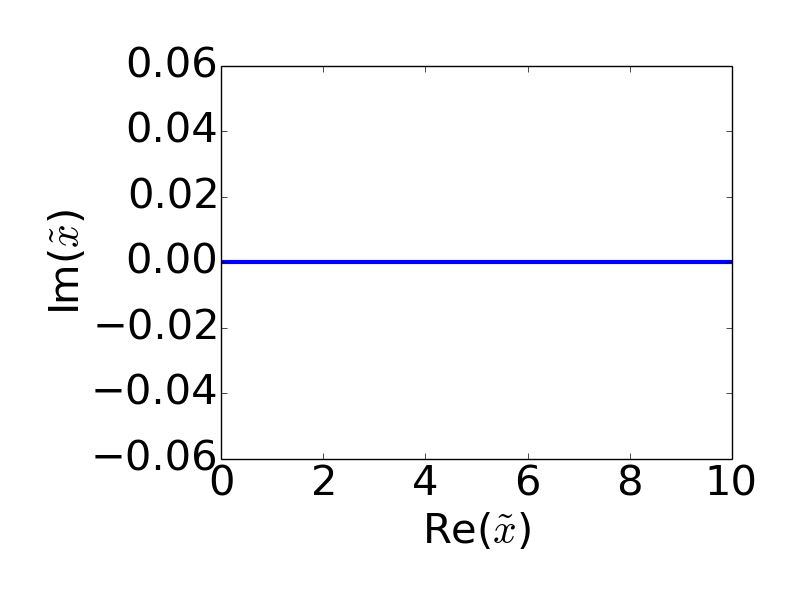
\includegraphics[width=\textwidth]{images/pml/real-x.png}
		\caption{}
	\end{subfigure}
	\begin{subfigure}{0.45\textwidth}
		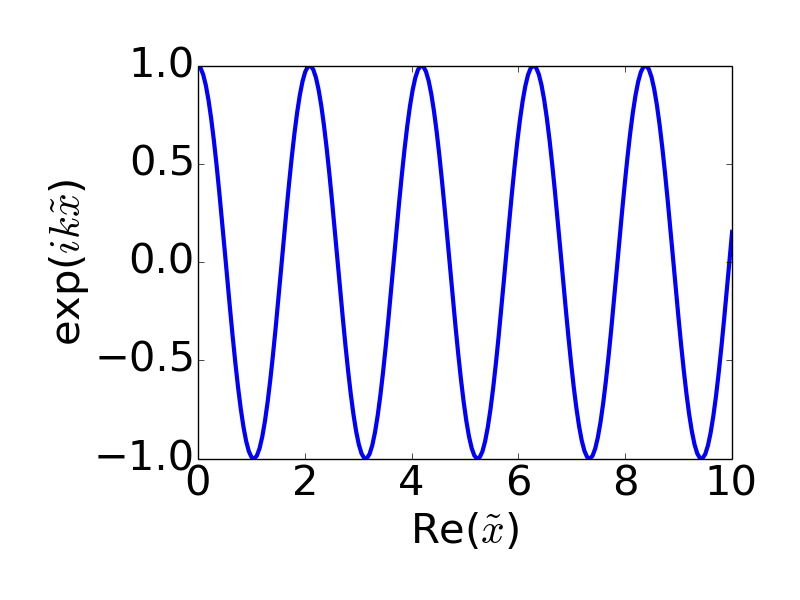
\includegraphics[width=\textwidth]{images/pml/real-x-wave.png}
		\caption{}
	\end{subfigure}


	\begin{subfigure}{0.45\textwidth}
		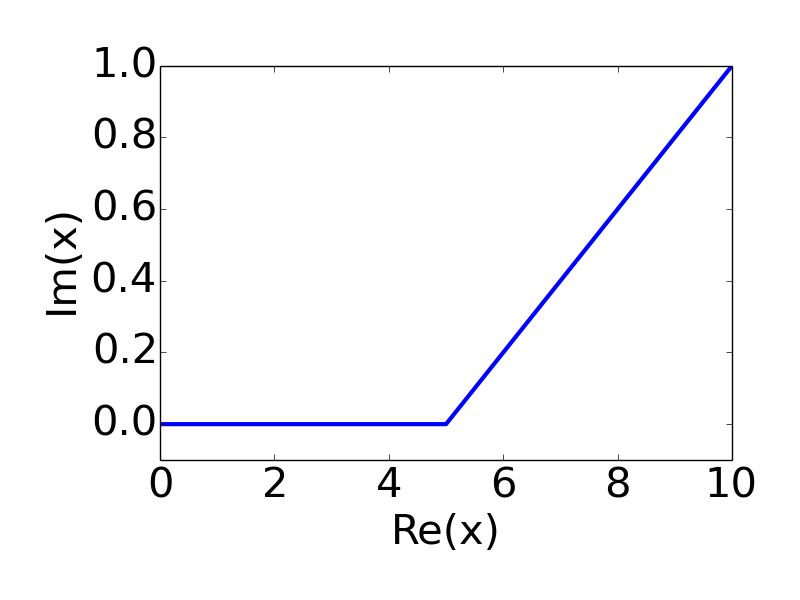
\includegraphics[width=\textwidth]{images/pml/complex-x.png}
		\caption{}
		\label{fig:complex-contour}
	\end{subfigure}
	\begin{subfigure}{0.45\textwidth}
		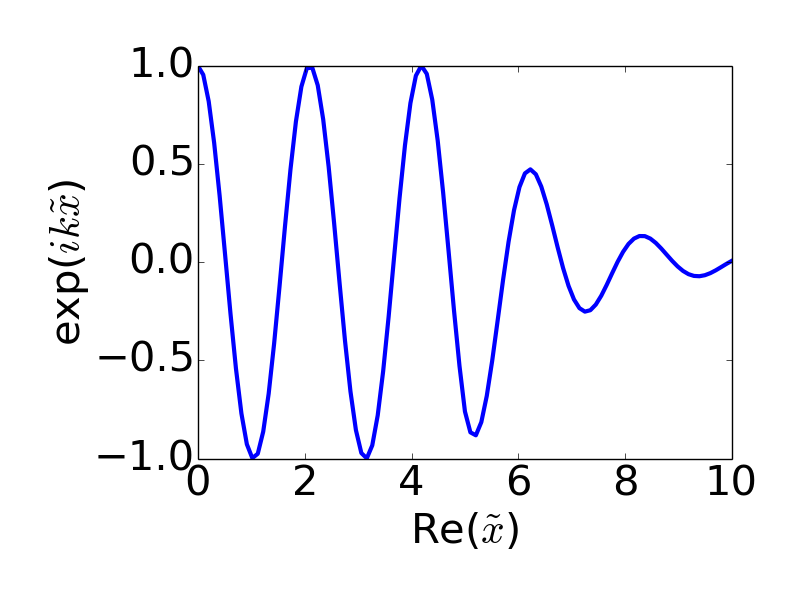
\includegraphics[width=\textwidth]{images/pml/complex-x-wave.png}
		\caption{}
		\label{fig:absorbing-region}
	\end{subfigure}

	\caption{Na rysunkach (a) i~(b) przedstawiono odpowiednio rzeczywiste wartości położenia na zespolonej płaszczyźnie $\tilde{x}$ i~odpowiadające im rozwiązanie równania falowego. Na rysunku (c) dla arbitralnej  wartości $\textrm{Re}(\tilde{x})>5$ przedstawiono zmieniony kontur wykorzystujący zespolone wartości dla $\tilde{x}$. Odpowiednie dla zmodyfikowanego konturu (c)  rozwiązanie równania falowego przedstawia wykres na rysunku (d).}
	\label{fig:var-transform}
\end{figure}


Kluczowym jest zauważenie, że składniki sumy z wzoru (\ref{eq:pml-cos}) mogą zostać zapisane w~postaci
\begin{equation}
\vec{W}(y,z)e^{i(k\tilde{x}-\omega t)},
\end{equation}
która to jest funkcją analityczną w~$\tilde{x}\in \mathbb{C}$. Oznacza to, że możemy dokonać jej analitycznego przedłużenia dla zespolonych wartości $x$. Falę propagującą, wraz z~czysto rzeczywistym konturem opisującym położenia w~kierunku $x$ przedstawiają wykresy na rysunku \ref{fig:var-transform}a i~\ref{fig:var-transform}b. 

Dla lepszego zrozumienia koncepcji rozważmy teraz zamianę zmiennych dla obszaru $x>x_0$, w taki sposób, że: 
\begin{equation}
\tilde{x}=  
\begin{cases} 
        x, & \mbox{dla } x< x_0 \\ 
        x+0.2x\mbox{ }i, & \mbox{dla } x>x_0 \\
\end{cases}.
\end{equation}
Rozwiązanie zagadnienia propagacji po takim zespolonym konturze dla $x_0=5$ przedstawia wykres na rysunku \ref{fig:complex-contour}. Zauważymy, że dla obszaru w~którym do rzeczywistej części dodaliśmy liniowo rosnącą część urojoną uzyskujemy falę zanikającą. Ponieważ na wykresie \ref{fig:absorbing-region} rozwiązanie dla $x<x_0$ nie uległo zmianie, a w~obszarze $x>x_0$ obserwujemy fale zanikającą to przestrzeń dla $x>x_0$ wykazuje działanie nieodbijającej warstwy absorpcyjnej.

\subsection{Wykorzystanie zamiany zmienny}

Zgodnie z przedstawionym przykładem rozwinięcie analityczne możemy dla wygody obliczeniowej traktować równoważnie z~zamianą współrzędnych w~omawianym równaniu różniczkowym. Oznaczmy zespoloną zmienną $\tilde{x}(x)=x+if(x)$, traktując od tej pory $x$ zawsze jako rzeczywiste położenie. Taka zamiana współrzędnych wymaga od nas zamiany każdego różniczkowania po zdeformowanym konturze $\partial \tilde{x} = (1+i\frac{df}{dx}) \partial x$. Ponieważ założyliśmy, że nasze równanie różniczkowe jest niezależne od x (przynajmniej dla dużych x, gdzie $f(x)\ne0$; wynika to bezpośrednio z~założenia jednorodności liniowości i~niezależności od czasu) nie musimy uwzględniać żadnych dodatkowych wyrazów. Jak wykażemy w~kolejnych akapitach wygodnie jest wybrać $\frac{df}{dx}=\frac{\sigma_x}{\omega}$ i~ostatecznie zapisać wymaganą zamianę zmiennych jako:
\begin{equation}
	\frac{\partial}{\partial \tilde{x}} \to \frac{1} {1+i \frac{\sigma_x(x)}{\omega}} \frac{\partial}{\partial x}.
	\label{eq:pml-variable-change}
\end{equation}

W obszarach PML, gdzie $\sigma_x\ne0$, oscylujące rozwiązania równania falowego przyjmują postać fal eksponencjalnie zanikających. Poza PML ( $\sigma_x=0$) rozwiązywane równanie pozostaje niezmienione: nie występują odbicia ponieważ jest to analityczne rozwinięcie pierwotnego rozwiązania i~w obszarach gdzie $\tilde{x}=x$ rozwiązanie nie może się zmienić.

Po wykonaniu podstawienia (\ref{eq:pml-variable-change}), rozwiązania równania falowego w~obszarze PML przyjmują postać:
\begin{equation}
e^{ikx}\textrm{exp}\Big(-\frac{k}{\omega}\int^x \sigma_x(x')dx'\Big).
\end{equation}
Warto zauważyć, że pojawiający się wykładnik potęgi $\frac{k}{\omega}$ dla materiałów bezdyspersyjnych jest stały i~równy odwrotności prędkości fazowej. W ten sposób uzasadniliśmy zaproponowany wybór $\frac{df}{dx}=\frac{\sigma_x}{\omega}$, dzięki któremu otrzymujemy niezależność współczynnika tłumienia od częstotliwości promieniowania E-M. 

\subsection{Wynik przeprowadzonej analizy}
Zgodnie z~przedstawionym wyprowadzeniem możemy zastosować dowolnie mały obszar PML, ponieważ nie ma żadnego ograniczenia na wartości $\sigma_x$. W praktyce numerycznej, ze względu na zastosowaną dyskretyzację gwałtowne zmiany $\sigma_x$ prowadzą do powstania ,,odbić numerycznych''. Z tego powodu $\sigma_x$ zazwyczaj ma postać funkcji kwadratowej lub sześciennej narastającej od zera do wartości maksymalnej na obszarze większym od połowy długości fali promieniowania występującego w~symulacji~\cite{johnson2008notes}.

W przypadku równań Maxwella każda zamiana współrzędnych może zostać wyrażona przez równania Maxwella we współrzędnych kartezjańskich ze zmienionymi materiałami~\cite{ward1996refraction}. Zamiana współrzędnych jest równoważna zmianie przenikalności elektrycznej $\varepsilon$ i~magnetycznej µ, w~ogólności na absorbujące ośrodki anizotropowe. 

W przypadku trójwymiarowych równań Maxwella dla ośrodka opisywanego za pomocą tensorów $\hat{\varepsilon}$ i~$\hat{\mu}$ 
\begin{equation}
\hat{\varepsilon}=
\begin{bmatrix}
\varepsilon_x & 0 & 0 \\
0 &\varepsilon_y & 0 \\
0 & 0  & \varepsilon_z  \\
\end{bmatrix}
, \hat{\mu}=
\begin{bmatrix}
\mu_x & 0 & 0 \\
0 &\mu_y & 0 \\
0 & 0  & \mu_z  \\
\end{bmatrix}
\end{equation}
warstwą PML może być materiał charakteryzujący się przenikalnością elektryczną i~magnetyczną opisywaną tensorami:
\begin{equation}
\hat{\varepsilon}_{\textrm{PML}}=
\begin{bmatrix}
s \cdot \varepsilon_x & 0 & 0 \\
0 &s \cdot \varepsilon_y & 0 \\
0 & 0  & \frac{ \varepsilon_z}{s}  \\
\end{bmatrix}
, \hat{\mu}_{\textrm{PML}}=
\begin{bmatrix}
s \cdot \mu_x & 0 & 0 \\
0 & s \cdot \mu_y & 0 \\
0 & 0  & \frac{\mu_z}{s}  \\
\end{bmatrix},
\label{eq:general-pml-form}
\end{equation}
gdzie $s$ jest dowolną liczbą zespoloną~\cite{sacks1995perfectly}, której część odpowiedzialna za tłumienie jest równoznaczna liniowemu współczynnikowi deformacji konturu zmiennych przestrzennych w~część urojoną.


